\documentclass[a4paper,12pt]{article}
\usepackage [left=25.4mm,top=25.4mm]{geometry}
\usepackage{amsmath}
\usepackage{amssymb}
\usepackage{graphicx}
%\usepackage{apacite}
\usepackage{url}
\usepackage{subfig}
\usepackage{csvsimple}
\usepackage{float}
\usepackage{lineno}
\usepackage[affil-it]{authblk}
\usepackage{setspace}
\usepackage{makecell} 
\usepackage{tikz}
\usepackage{csvsimple}
\usepackage{newfloat}
\usepackage{xcolor}
\usepackage{tabularx,booktabs}
\usepackage{multirow}
\usepackage{multicol}
\usepackage{array}
\usepackage{tocbasic}
\usepackage{sectsty}

\sectionfont{\fontsize{12}{15}\selectfont}
\chapterfont{\fontsize{14}{15}\selectfont}
\subsectionfont{\fontsize{10}{15}\selectfont}

\newcommand\hcancel[2][black]{\setbox0=\hbox{$#2$}%
	\rlap{\raisebox{.45\ht0}{\textcolor{#1}{\rule{\wd0}{1pt}}}}#2} 
\newcommand{\forceindent}{\leavevmode{\parindent=2em\indent}}

\DeclareFloatingEnvironment[name={Supplementary Figure},fileext=lsf,listname={List of Supplementary Figures}]{suppfigure}
\DeclareFloatingEnvironment[name={Supplementary Table},fileext=lsf,listname={List of Supplementary Tables}]{supptable}
\DeclareFloatingEnvironment[name={Supplementary Material},fileext=lsf,listname={List of Supplementary Material}]{suppmat}

\newcolumntype{P}[1]{>{\centering\arraybackslash}p{#1}}
\newcolumntype{M}[1]{>{\centering\arraybackslash}m{#1}}

\DeclareMathOperator*{\argmax}{arg\,max}
\DeclareMathOperator*{\argmin}{arg\,min}

\newcommand{\indep}{\perp \!\!\! \perp}
\renewcommand*\contentsname{TABLE OF CONTENTS}
\renewcommand{\listfigurename}{LIST OF FIGURES}
\renewcommand{\listtablename}{LIST OF TABLES}

\renewcommand{\arraystretch}{1.5}
\begin{document}
	\begin{titlepage}
		\title{Modularity Examples}
		\author[1]{Jarred M. Kvamme}
		\affil[1]{Department of Bioinformatics and Computational Biology - University of Idaho}
		\maketitle
	\end{titlepage}
	
	
	\newpage
	\tableofcontents{}
	\addcontentsline{toc}{section}{LIST OF TABLES}
	\addcontentsline{toc}{section}{LIST OF FIGURES}
	\listoftables
	\listoffigures
	\newpage
	
	\section{The Case of two completely disconnected communities}
	In this first example, we explore how modularity is affected by exploring the modularity for two completely disconnected sub-networks and comparing when the sub-networks are merged into a single community.
	\begin{figure}[H]
		\centering
		\caption{Case 1 graph}
		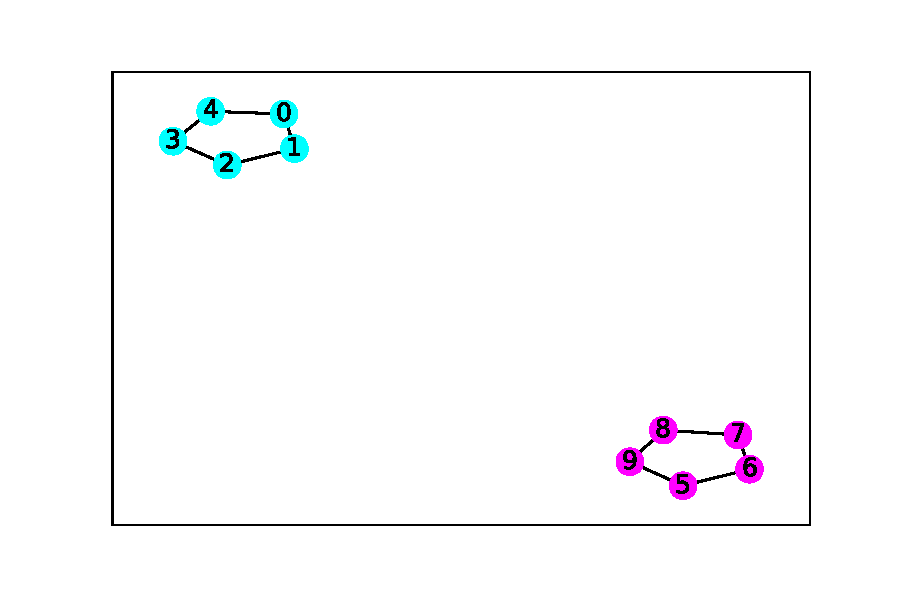
\includegraphics[scale=0.65]{C:/Users/Bruin/Documents/GitHub/HGRN_repo/Modularity/case1_2clusts.pdf}
		\label{fig:case1}
	\end{figure}
	\subsection*{Modularity for two communities of 5 nodes}
	Let $\bf{C}$ be the the community assignment matrix 
	\[ {\bf C} = \begin{bmatrix}1 & 0 \\ 1 & 0 \\ 1 & 0 \\ 1 & 0 \\ 1 & 0 \\ 1 & 0 \\ 0 & 1 \\ 0 & 1 \\ 0 & 1 \\ 0 & 1 \\ 0 & 1 \\
	\end{bmatrix}\] 
	
	Let $\bf A$ be the graph adjacency matrix
	\[ {\bf A} = \begin{bmatrix}
		0& 1& 0& 0& 1& 0& 0& 0& 0& 0\\
		1& 0& 1& 0& 0& 0& 0& 0& 0& 0\\
		0& 1& 0& 1& 0& 0& 0& 0& 0& 0\\
		0& 0& 1& 0& 1& 0& 0& 0& 0& 0\\
		1& 0& 0& 1& 0& 0& 0& 0& 0& 0\\
		0& 0& 0& 0& 0& 0& 1& 0& 0& 1\\
		0& 0& 0& 0& 0& 1& 0& 1& 0& 0\\
		0& 0& 0& 0& 0& 0& 1& 0& 1& 0\\
		0& 0& 0& 0& 0& 0& 0& 1& 0& 1\\
		0& 0& 0& 0& 0& 1& 0& 0& 1& 0
	\end{bmatrix}\] 
	
	Further let $\bf B$ be the modularity matrix defined as 
	
	\[ {\bf B} = {\bf A} - \frac{1}{2m}{\bf r}\otimes {\bf r} \]
	
	where 
	
	\[ {\bf r} = \begin{bmatrix}
		0& 1& 0& 0& 1& 0& 0& 0& 0& 0\\
		1& 0& 1& 0& 0& 0& 0& 0& 0& 0\\
		0& 1& 0& 1& 0& 0& 0& 0& 0& 0\\
		0& 0& 1& 0& 1& 0& 0& 0& 0& 0\\
		1& 0& 0& 1& 0& 0& 0& 0& 0& 0\\
		0& 0& 0& 0& 0& 0& 1& 0& 0& 1\\
		0& 0& 0& 0& 0& 1& 0& 1& 0& 0\\
		0& 0& 0& 0& 0& 0& 1& 0& 1& 0\\
		0& 0& 0& 0& 0& 0& 0& 1& 0& 1\\
		0& 0& 0& 0& 0& 1& 0& 0& 1& 0
	\end{bmatrix} \cdot \begin{bmatrix}
	1 & \\ 1 & \\ 1 & \\ 1 & \\ 1 & \\ 1 & \\ 1 & \\ 1 & \\ 1 & \\ 1 & \\
	\end{bmatrix} = \begin{bmatrix}
	2 & \\ 2 & \\ 2 & \\ 2 & \\ 2 & \\ 2 & \\ 2 & \\ 2 & \\ 2 & \\ 2 & \\
	\end{bmatrix} \]
	
	therefore
	
	\[ {\bf r}\otimes {\bf r} = \begin{bmatrix}
		4& 4& 4& 4& 4& 4& 4& 4& 4& 4\\
		4& 4& 4& 4& 4& 4& 4& 4& 4& 4\\
		4& 4& 4& 4& 4& 4& 4& 4& 4& 4\\
		4& 4& 4& 4& 4& 4& 4& 4& 4& 4\\
		4& 4& 4& 4& 4& 4& 4& 4& 4& 4\\
		4& 4& 4& 4& 4& 4& 4& 4& 4& 4\\
		4& 4& 4& 4& 4& 4& 4& 4& 4& 4\\
		4& 4& 4& 4& 4& 4& 4& 4& 4& 4\\
		4& 4& 4& 4& 4& 4& 4& 4& 4& 4\\
		4& 4& 4& 4& 4& 4& 4& 4& 4& 4
	\end{bmatrix}\]
	
	we also have that 
	
	\[ m = \frac{1}{2} \sum_i \sum_j {\bf A}_{i,j} = 10\]
	
	therefore the modularity matrix can be expressed as 
	\[ {\bf B} = \begin{bmatrix}
		-\frac{4}{20}& \frac{16}{20}& -\frac{4}{20}& -\frac{4}{20}& \frac{16}{20}& -\frac{4}{20}& -\frac{4}{20}& -\frac{4}{20}& -\frac{4}{20}& -\frac{4}{20}\\
		\frac{16}{20}& -\frac{4}{20}& \frac{16}{20}& -\frac{4}{20}& -\frac{4}{20}& -\frac{4}{20}& -\frac{4}{20}& -\frac{4}{20}& -\frac{4}{20}& -\frac{4}{20}\\
		-\frac{4}{20}& \frac{16}{20}& -\frac{4}{20}& \frac{16}{20}& -\frac{4}{20}& -\frac{4}{20}& -\frac{4}{20}& -\frac{4}{20}& -\frac{4}{20}& -\frac{4}{20}\\
		-\frac{4}{20}& -\frac{4}{20}& \frac{16}{20}& -\frac{4}{20}& \frac{16}{20}& -\frac{4}{20}& -\frac{4}{20}& -\frac{4}{20}& -\frac{4}{20}& -\frac{4}{20}\\
		\frac{16}{20}& -\frac{4}{20}& -\frac{4}{20}& \frac{16}{20}& -\frac{4}{20}& -\frac{4}{20}& -\frac{4}{20}& -\frac{4}{20}& -\frac{4}{20}& -\frac{4}{20}\\
		-\frac{4}{20}& -\frac{4}{20}& -\frac{4}{20}& -\frac{4}{20}& -\frac{4}{20}& -\frac{4}{20}& \frac{16}{20}& -\frac{4}{20}& -\frac{4}{20}& \frac{16}{20}\\
		-\frac{4}{20}& -\frac{4}{20}& -\frac{4}{20}& -\frac{4}{20}& -\frac{4}{20}& \frac{16}{20}& -\frac{4}{20}& \frac{16}{20}& -\frac{4}{20}& -\frac{4}{20}\\
		-\frac{4}{20}& -\frac{4}{20}& -\frac{4}{20}& -\frac{4}{20}& -\frac{4}{20}& -\frac{4}{20}& \frac{16}{20}& -\frac{4}{20}& \frac{16}{20}& -\frac{4}{20}\\
		-\frac{4}{20}& -\frac{4}{20}& -\frac{4}{20}& -\frac{4}{20}& -\frac{4}{20}& -\frac{4}{20}& -\frac{4}{20}& \frac{16}{20}& -\frac{4}{20}& \frac{16}{20}\\
		-\frac{4}{20}& -\frac{4}{20}& -\frac{4}{20}& -\frac{4}{20}& -\frac{4}{20}& \frac{16}{20}& -\frac{4}{20}& -\frac{4}{20}& \frac{16}{20}& -\frac{4}{20}
	\end{bmatrix} \]
	
	We compute the modularity using the following equation
	
	\[M = \frac{1}{4m}Tr({\bf C^T B C}) \]
	
	where 
	\[ {\bf C^T B C} = \] 
	\[\small \begin{bmatrix}
		1 & 1 & 1 & 1 & 1 & 0 & 0 & 0 & 0 & 0 \\
		0 & 0 & 0 & 0 & 0 & 1 & 1 & 1 & 1 & 1 \\
	\end{bmatrix}\cdot  \begin{bmatrix}
		-\frac{4}{20}& \frac{16}{20}& -\frac{4}{20}& -\frac{4}{20}& \frac{16}{20}& -\frac{4}{20}& -\frac{4}{20}& -\frac{4}{20}& -\frac{4}{20}& -\frac{4}{20}\\
		\frac{16}{20}& -\frac{4}{20}& \frac{16}{20}& -\frac{4}{20}& -\frac{4}{20}& -\frac{4}{20}& -\frac{4}{20}& -\frac{4}{20}& -\frac{4}{20}& -\frac{4}{20}\\
		-\frac{4}{20}& \frac{16}{20}& -\frac{4}{20}& \frac{16}{20}& -\frac{4}{20}& -\frac{4}{20}& -\frac{4}{20}& -\frac{4}{20}& -\frac{4}{20}& -\frac{4}{20}\\
		-\frac{4}{20}& -\frac{4}{20}& \frac{16}{20}& -\frac{4}{20}& \frac{16}{20}& -\frac{4}{20}& -\frac{4}{20}& -\frac{4}{20}& -\frac{4}{20}& -\frac{4}{20}\\
		\frac{16}{20}& -\frac{4}{20}& -\frac{4}{20}& \frac{16}{20}& -\frac{4}{20}& -\frac{4}{20}& -\frac{4}{20}& -\frac{4}{20}& -\frac{4}{20}& -\frac{4}{20}\\
		-\frac{4}{20}& -\frac{4}{20}& -\frac{4}{20}& -\frac{4}{20}& -\frac{4}{20}& -\frac{4}{20}& \frac{16}{20}& -\frac{4}{20}& -\frac{4}{20}& \frac{16}{20}\\
		-\frac{4}{20}& -\frac{4}{20}& -\frac{4}{20}& -\frac{4}{20}& -\frac{4}{20}& \frac{16}{20}& -\frac{4}{20}& \frac{16}{20}& -\frac{4}{20}& -\frac{4}{20}\\
		-\frac{4}{20}& -\frac{4}{20}& -\frac{4}{20}& -\frac{4}{20}& -\frac{4}{20}& -\frac{4}{20}& \frac{16}{20}& -\frac{4}{20}& \frac{16}{20}& -\frac{4}{20}\\
		-\frac{4}{20}& -\frac{4}{20}& -\frac{4}{20}& -\frac{4}{20}& -\frac{4}{20}& -\frac{4}{20}& -\frac{4}{20}& \frac{16}{20}& -\frac{4}{20}& \frac{16}{20}\\
		-\frac{4}{20}& -\frac{4}{20}& -\frac{4}{20}& -\frac{4}{20}& -\frac{4}{20}& \frac{16}{20}& -\frac{4}{20}& -\frac{4}{20}& \frac{16}{20}& -\frac{4}{20}
	\end{bmatrix} \cdot 
	\begin{bmatrix}
	1 & 0 \\ 
	1 & 0 \\
	1 & 0 \\
	1 & 0 \\ 
	1 & 0 \\ 
	1 & 0 \\ 
	0 & 1 \\ 
	0 & 1 \\ 
	0 & 1 \\ 
	0 & 1 \\ 
	0 & 1 
	\end{bmatrix}\]
	
		\[\small =\begin{bmatrix}
		1&  1&  1&  1&  1& -1& -1& -1& -1& -1 \\
	   -1& -1& -1& -1& -1&  1&  1&  1&  1&  1 \\
	\end{bmatrix} \cdot 
	\begin{bmatrix}
		1 & 0 \\ 
		1 & 0 \\
		1 & 0 \\
		1 & 0 \\ 
		1 & 0 \\ 
		1 & 0 \\ 
		0 & 1 \\ 
		0 & 1 \\ 
		0 & 1 \\ 
		0 & 1 \\ 
		0 & 1 
	\end{bmatrix}\]
	
	
	\[ =\begin{bmatrix}
		5 & -5 \\
		-5 & 5 \\
	\end{bmatrix} \]
	
	Therefore the modularity equals 
	
	\[ M = \frac{1}{40} \times Tr\left( \begin{bmatrix}
		5 & -5 \\
		-5 & 5 \\
	\end{bmatrix} \right) \]
	
	\[ = \frac{1}{40} \times 10 = 0.25\]
	
	\subsection*{Modularity for a single community of 10 nodes}
	In our second example we compute the modularity when all of the nodes are grouped into a single cluster. The only computation which we much change is ${\bf C^T B C}$. In this scenario, the community assignment matrix is as follows
	
	\[ {\bf C} = \begin{bmatrix}1 & 0 \\ 1 & 0 \\ 1 & 0 \\ 1 & 0 \\ 1 & 0 \\ 1 & 0 \\ 1 & 0 \\ 1 & 0 \\ 1 & 0 \\ 1 & 0 \\ 1 & 0 \\
	\end{bmatrix}\] 
	
	
	\[ {\bf C^T B C} = \] 
	\[\small \begin{bmatrix}
		1 & 1 & 1 & 1 & 1 & 1 & 1 & 1 & 1 & 1 \\
		0 & 0 & 0 & 0 & 0 & 0 & 0 & 0 & 0 & 0 \\
	\end{bmatrix}\cdot  \begin{bmatrix}
		-\frac{4}{20}& \frac{16}{20}& -\frac{4}{20}& -\frac{4}{20}& \frac{16}{20}& -\frac{4}{20}& -\frac{4}{20}& -\frac{4}{20}& -\frac{4}{20}& -\frac{4}{20}\\
		\frac{16}{20}& -\frac{4}{20}& \frac{16}{20}& -\frac{4}{20}& -\frac{4}{20}& -\frac{4}{20}& -\frac{4}{20}& -\frac{4}{20}& -\frac{4}{20}& -\frac{4}{20}\\
		-\frac{4}{20}& \frac{16}{20}& -\frac{4}{20}& \frac{16}{20}& -\frac{4}{20}& -\frac{4}{20}& -\frac{4}{20}& -\frac{4}{20}& -\frac{4}{20}& -\frac{4}{20}\\
		-\frac{4}{20}& -\frac{4}{20}& \frac{16}{20}& -\frac{4}{20}& \frac{16}{20}& -\frac{4}{20}& -\frac{4}{20}& -\frac{4}{20}& -\frac{4}{20}& -\frac{4}{20}\\
		\frac{16}{20}& -\frac{4}{20}& -\frac{4}{20}& \frac{16}{20}& -\frac{4}{20}& -\frac{4}{20}& -\frac{4}{20}& -\frac{4}{20}& -\frac{4}{20}& -\frac{4}{20}\\
		-\frac{4}{20}& -\frac{4}{20}& -\frac{4}{20}& -\frac{4}{20}& -\frac{4}{20}& -\frac{4}{20}& \frac{16}{20}& -\frac{4}{20}& -\frac{4}{20}& \frac{16}{20}\\
		-\frac{4}{20}& -\frac{4}{20}& -\frac{4}{20}& -\frac{4}{20}& -\frac{4}{20}& \frac{16}{20}& -\frac{4}{20}& \frac{16}{20}& -\frac{4}{20}& -\frac{4}{20}\\
		-\frac{4}{20}& -\frac{4}{20}& -\frac{4}{20}& -\frac{4}{20}& -\frac{4}{20}& -\frac{4}{20}& \frac{16}{20}& -\frac{4}{20}& \frac{16}{20}& -\frac{4}{20}\\
		-\frac{4}{20}& -\frac{4}{20}& -\frac{4}{20}& -\frac{4}{20}& -\frac{4}{20}& -\frac{4}{20}& -\frac{4}{20}& \frac{16}{20}& -\frac{4}{20}& \frac{16}{20}\\
		-\frac{4}{20}& -\frac{4}{20}& -\frac{4}{20}& -\frac{4}{20}& -\frac{4}{20}& \frac{16}{20}& -\frac{4}{20}& -\frac{4}{20}& \frac{16}{20}& -\frac{4}{20}
	\end{bmatrix} \cdot 
	\begin{bmatrix}
		1 & 0 \\ 
		1 & 0 \\
		1 & 0 \\
		1 & 0 \\ 
		1 & 0 \\ 
		1 & 0 \\ 
		1 & 0 \\ 
		1 & 0 \\ 
		1 & 0 \\ 
		1 & 0 \\ 
		1 & 0 
	\end{bmatrix}\]
	
	\[\small =\begin{bmatrix}
		0&  0&  0&  0&  0& 0& 0& 0& 0& 0 \\
		0& 0& 0& 0& 0& 0& 0& 0& 0&  0 \\
	\end{bmatrix} \cdot 
	\begin{bmatrix}
		1 & 0 \\ 
		1 & 0 \\
		1 & 0 \\
		1 & 0 \\ 
		1 & 0 \\ 
		1 & 0 \\ 
		1 & 0 \\ 
		1 & 0 \\ 
		1 & 0 \\ 
		1 & 0 \\ 
		1 & 0 
	\end{bmatrix}\]
	
	
	\[ =\begin{bmatrix}
		0 & 0 \\
		0 & 0 \\
	\end{bmatrix} \]
	
	\[M = \frac{1}{40} \times 0 = 0\]
	
	
	\newpage
	\section{The Case of a network divided into 2 communities}
	
	\begin{figure}[H]
		\centering
		\caption{Case 1 graph}
		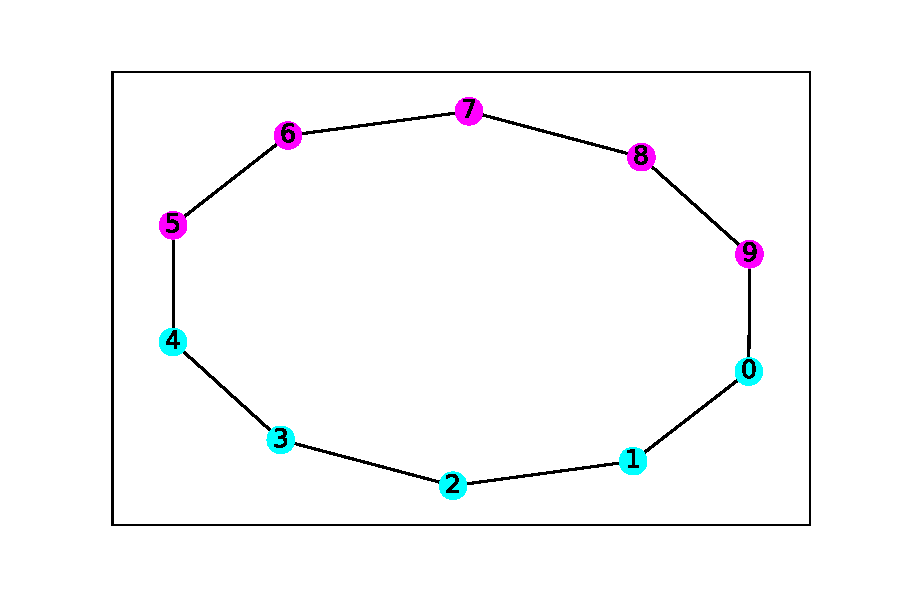
\includegraphics[scale=0.65]{C:/Users/Bruin/Documents/GitHub/HGRN_repo/Modularity/on_net_multi_comms.pdf}
		\label{fig:case2}
	\end{figure}
	
	
	
	
	
	
	
	
	
	
	
	
	
	
	
	
	
	
	
	
	
	
	
	
	
	
	
	
	\newpage
		\section{The Case of a singleton community}
	In this second example, we explore how modularity is affected by the presence of a singleton community in a two community graph. Specifically, we explore how modularity changes when from two communities where one community consists of a single isolated node (singleton) and the other community consists of a community of 10 nodes. We two cases for the non-singleton community (i) when all 10-nodes are fully connected vs when all 10 nodes come from a Wattz Strogratz graph with degree 2. 	
	
	\[ {\bf C} = \begin{bmatrix}1 & 0 \\ 1 & 0 \\ 1 & 0 \\ 1 & 0 \\ 1 & 0 \\ 0 & 1 \\	\end{bmatrix}\] 
	
	Let $\bf A$ be the graph adjacency matrix
	\[ {\bf A} = \begin{bmatrix}
		0& 1& 0& 0& 1& 0 \\
		1& 0& 1& 0& 0& 0 \\
		0& 1& 0& 1& 0& 0 \\
		0& 0& 1& 0& 1& 0 \\
		1& 0& 0& 1& 0& 0 \\
		0& 0& 0& 0& 0& 0 \\
	\end{bmatrix}\] 
	
	
	\begin{figure}[H]
		\centering
		\caption{Case 2 graph}
		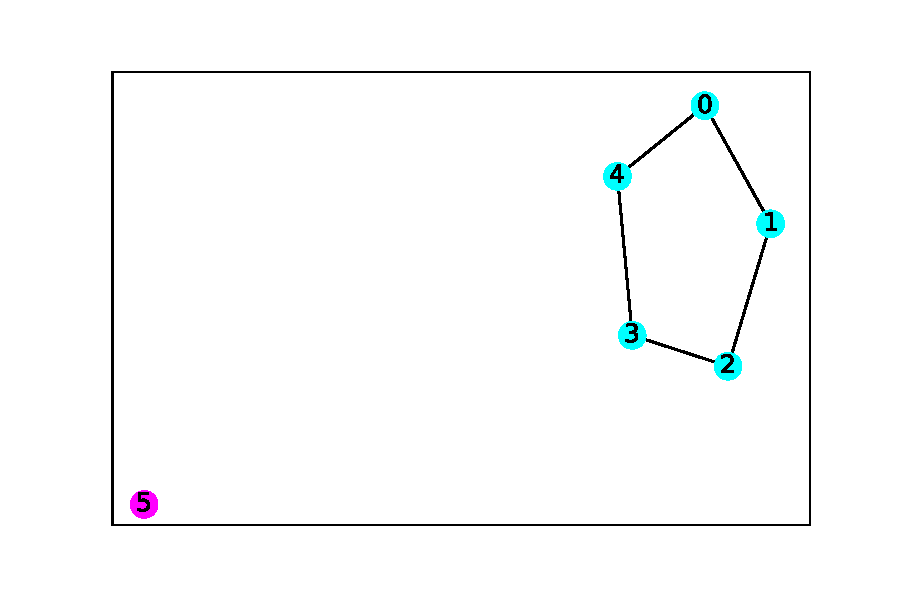
\includegraphics[scale=0.65]{C:/Users/Bruin/Documents/GitHub/HGRN_repo/Modularity/case2_singleton.pdf}
		\label{fig:case3}
	\end{figure}
	
	
	
	
	
	
	
	
	
	
	
	
	
	
	
	
	
	
	
	
	
	
	
	
	
	
	
	
	
	
	
	
	
	
	\clearpage
	\newpage
	
	\bibliographystyle{unsrt}
	\bibliography{pseudocode_bibs}
	
	
	
	
	
	
\end{document}